\documentclass{article}

% Language setting
% Replace `english' with e.g. `spanish' to change the document language
\usepackage[english]{babel}

% Set page size and margins
% Replace `letterpaper' with `a4paper' for UK/EU standard size
\usepackage[letterpaper,top=2cm,bottom=2cm,left=3cm,right=3cm,marginparwidth=1.75cm]{geometry}

% Useful packages
\usepackage{amsmath}
\usepackage{graphicx}
\usepackage[colorlinks=true, allcolors=blue]{hyperref}
\usepackage{tikz}
\usetikzlibrary{shapes,arrows,positioning}
\usepackage{booktabs}

% Title
\title{Implementing RaptorQ in Hadoop\\
\large ICT3 Project n°1 — Shanghai Jiao Tong University}
\author{Alexandra Baron \and Mathis Liens \and Charles Pelong\and Baptiste Halçaren \and Maria Stivala \and Arnaud Brisset}
\date{October 2025}

\begin{document}
\maketitle

% University logo - Placed AFTER title and smaller
\begin{figure}[htbp]
\centering
\includegraphics[width=0.4\linewidth]{images/shanghai-jiao-tong-university.png}
\end{figure}

\begin{abstract}
This report presents the implementation of RaptorQ erasure coding as an alternative to Reed-Solomon in Hadoop 3.4.2. We leverage the OpenRQ library, an open-source RFC 6330 RaptorQ implementation, and integrate it into Hadoop's three-layer erasure coding architecture. Our implementation adapts RaptorQ's fountain code model to Hadoop's fixed-parity requirements through deterministic ESI mapping and parity regeneration strategies. Comprehensive unit tests validate encoding and decoding correctness across various erasure scenarios. This work demonstrates the extensibility of Hadoop's erasure coding framework while providing insights into the trade-offs between deterministic and probabilistic erasure coding approaches.
\end{abstract}

\section{Introduction}

Distributed storage systems face the challenge of maintaining data durability and availability in the presence of node failures. Traditional replication strategies, while simple, incur significant storage overhead. Erasure coding (EC) provides a storage-efficient alternative by encoding data into $k$ data blocks and $m$ parity blocks, allowing reconstruction of the original data from any $k$ out of $k+m$ blocks.

Hadoop 3.x introduced erasure coding support, with Reed-Solomon (RS) as the primary algorithm. While RS is deterministic and well-understood, it has limitations in certain scenarios, particularly in streaming applications where fountain codes like RaptorQ offer advantages.

This project aims to implement RaptorQ erasure coding in Hadoop 3.4.2, providing an alternative to Reed-Solomon that offers probabilistic decoding and the ability to generate an unlimited number of repair symbols. The implementation integrates the OpenRQ library, a Java implementation of RFC 6330 RaptorQ, into Hadoop's existing erasure coding framework.

\section{Background and Motivation}

\subsection{Erasure Coding in Hadoop}

Hadoop implements a three-layer erasure coding architecture that separates concerns and enables extensibility. Table \ref{tab:comparison} provides a comparison between Reed-Solomon and RaptorQ approaches.

\begin{table}[h]
\centering
\begin{tabular}{|p{5cm}|p{5cm}|}
\hline
\textbf{Reed-Solomon} & \textbf{RaptorQ} \\\hline
Deterministic (exact $k$ symbols) & Fountain code ($k+\epsilon$ symbols) \\\hline
Finite field arithmetic (GF256) & LT code + pre-coding \\\hline
Fixed $m$ parity symbols & Unlimited repair symbols \\\hline
Well-optimized native implementations & Moderate performance (Java) \\\hline
Always succeeds with $k$ symbols & Probabilistic (rare failures) \\\hline
\end{tabular}
\caption{\label{tab:comparison}Key differences between Reed-Solomon and RaptorQ}
\end{table}

Hadoop's current architecture expects exactly $m$ parity blocks, requiring adaptation of RaptorQ's unlimited symbol generation model while preserving its fountain code properties.

\section{Hadoop Erasure Coding Architecture}

Hadoop's erasure coding follows a three-layer architecture that separates concerns and enables extensibility. Figure \ref{fig:layers} illustrates this layered structure:

\begin{figure}[h]
\centering
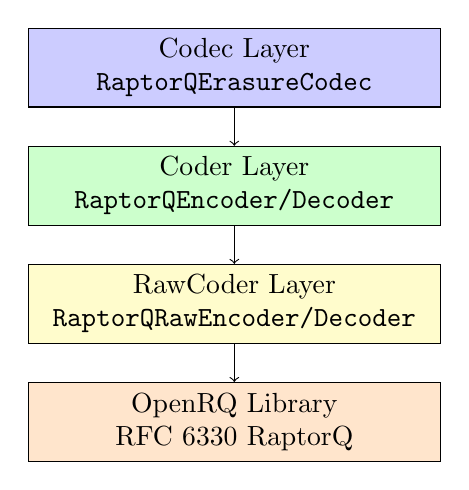
\begin{tikzpicture}[node distance=1.5cm, auto]
    % Codec Layer
    \node[rectangle, draw, fill=blue!20, text width=5cm, text centered, minimum height=1cm] (codec) {Codec Layer\\\texttt{RaptorQErasureCodec}};
    
    % Coder Layer
    \node[rectangle, draw, fill=green!20, text width=5cm, text centered, minimum height=1cm, below of=codec] (coder) {Coder Layer\\\texttt{RaptorQEncoder/Decoder}};
    
    % RawCoder Layer
    \node[rectangle, draw, fill=yellow!20, text width=5cm, text centered, minimum height=1cm, below of=coder] (rawcoder) {RawCoder Layer\\\texttt{RaptorQRawEncoder/Decoder}};
    
    % OpenRQ Library
    \node[rectangle, draw, fill=orange!20, text width=5cm, text centered, minimum height=1cm, below of=rawcoder] (openrq) {OpenRQ Library\\RFC 6330 RaptorQ};
    
    % Arrows
    \draw[->] (codec) -- (coder);
    \draw[->] (coder) -- (rawcoder);
    \draw[->] (rawcoder) -- (openrq);
\end{tikzpicture}
\caption{\label{fig:layers}Hadoop three-layer erasure coding architecture with RaptorQ integration}
\end{figure}

\begin{itemize}
\item \textbf{Codec Layer} (\texttt{codec/}): Defines high-level codec interfaces. Each codec (\texttt{ErasureCodec}) specifies the erasure schema $(k, m)$ and creates encoders/decoders. We implemented \texttt{RaptorQErasureCodec} following the pattern of existing codecs like \texttt{RSErasureCodec} and \texttt{XORErasureCodec}.

\item \textbf{Coder Layer} (\texttt{coder/}): Orchestrates encoding/decoding operations and manages block groups. \texttt{ErasureEncoder} and \texttt{ErasureDecoder} prepare input/output blocks and delegate to raw coders. Our \texttt{RaptorQEncoder} and \texttt{RaptorQDecoder} handle Hadoop-specific block management.

\item \textbf{RawCoder Layer} (\texttt{rawcoder/}): Implements the mathematical algorithms. \texttt{RawErasureEncoder} and \texttt{RawErasureDecoder} operate directly on byte arrays and ByteBuffers, performing pure computations. Our \texttt{RaptorQRawEncoder} and \texttt{RaptorQRawDecoder} integrate with the OpenRQ library.
\end{itemize}

The architecture uses Java's \texttt{ServiceLoader} mechanism for automatic factory discovery. Raw coder factories are registered in \texttt{META-INF/services/org.apache.hadoop.io.erasurecode.rawcoder.RawErasureCoderFactory}, enabling automatic discovery and fallback mechanisms. Configuration maps codec names to classes via \texttt{io.erasurecode.codec.raptorq}.

\section{RaptorQ and OpenRQ Library}

RaptorQ (RFC 6330) is a fountain code that encodes data into fixed-size symbols and can generate an unlimited number of repair symbols. Unlike Reed-Solomon which requires exactly $k$ symbols, RaptorQ can reconstruct data from any $k$ independent symbols (source or repair) with high probability. The algorithm guarantees success with $k+\epsilon$ symbols where $\epsilon$ is typically very small (often zero in practice).

OpenRQ is the Java implementation we used. Its key classes include:
\begin{itemize}
\item \texttt{FECParameters}: Encapsulates encoding parameters (data length, symbol size, number of source blocks)
\item \texttt{DataEncoder/DataDecoder}: High-level encoding/decoding interfaces
\item \texttt{SourceBlockEncoder/SourceBlockDecoder}: Per-block encoding/decoding operations
\item \texttt{EncodingPacket}: Transmittable packet structure containing symbol data and metadata
\end{itemize}

\subsection{Adaptation to Hadoop's Fixed-Parity Model}

The primary challenge is adapting RaptorQ's unlimited symbol generation model to Hadoop's requirement of exactly $m$ parity blocks. We solve this through deterministic Encoding Symbol Identifier (ESI) mapping:

\begin{table}[h]
\centering
\begin{tabular}{l|c|c}
\hline
\textbf{Hadoop Block} & \textbf{RaptorQ ESI} & \textbf{Symbol Type} \\\hline
Data block 0 & ESI 0 & Source symbol \\
Data block 1 & ESI 1 & Source symbol \\
\ldots & \ldots & \ldots \\
Data block $k-1$ & ESI $k-1$ & Source symbol \\\hline
Parity block 0 & ESI $k$ & Repair symbol \\
Parity block 1 & ESI $k+1$ & Repair symbol \\
\ldots & \ldots & \ldots \\
Parity block $m-1$ & ESI $k+m-1$ & Repair symbol \\\hline
\end{tabular}
\caption{\label{tab:esi-mapping}ESI mapping between Hadoop blocks and RaptorQ symbols}
\end{table}

This deterministic mapping ensures that the same input always produces the same parity output, which is crucial for Hadoop's block management and consistency requirements.

\section{Implementation}

\subsection{Architecture Integration}

Our implementation follows Hadoop's three-layer architecture:

\begin{itemize}
\item \textbf{Codec Layer}: \texttt{RaptorQErasureCodec} extends \texttt{ErasureCodec} and creates \texttt{RaptorQEncoder} and \texttt{RaptorQDecoder} instances. It registers the codec name \texttt{"raptorq"} in \texttt{ErasureCodeConstants}.

\item \textbf{Coder Layer}: \texttt{RaptorQEncoder} and \texttt{RaptorQDecoder} extend their respective base classes and delegate to raw coders via \texttt{CodecUtil.createRawEncoder/Decoder()}. They handle Hadoop block group management while the raw coders perform mathematical operations.

\item \textbf{RawCoder Layer}: \texttt{RaptorQRawEncoder} and \texttt{RaptorQRawDecoder} implement the integration with OpenRQ, performing the actual encoding and decoding computations.
\end{itemize}

\subsection{Encoding Process}

The encoding process follows these steps:

\begin{enumerate}
\item Concatenate $k$ input data chunks (each of size $T$) into a single buffer of size $k \times T$ bytes
\item Create \texttt{FECParameters} with data length $k \times T$, symbol size $T$, and one source block
\item Initialize OpenRQ \texttt{DataEncoder} and \texttt{SourceBlockEncoder}
\item Generate $m$ repair symbols with ESIs $k$ through $k+m-1$ (deterministic selection)
\item Write each repair symbol to the corresponding parity output
\end{enumerate}

\subsection{Decoding Process}

The decoding process handles both data and parity block recovery:

\begin{enumerate}
\item Build \texttt{FECParameters} matching the encoding parameters
\item Create OpenRQ \texttt{DataDecoder} and \texttt{SourceBlockDecoder}
\item Feed all available symbols (data and parity) to the decoder as \texttt{EncodingPacket}s
\item Once decoding succeeds, extract recovered data symbols for erased data blocks
\item For erased parity blocks, regenerate them by re-encoding the recovered data (since the decoder only provides source symbols)
\end{enumerate}

\subsection{Implementation Details}

We support both \texttt{byte[]} and \texttt{ByteBuffer} APIs for performance optimization. The ByteBuffer path enables zero-copy operations in some scenarios, while the byte array path provides simplicity and compatibility.

ServiceLoader registration makes the factory discoverable as \texttt{raptorq\_java}. We added a built-in erasure coding policy \texttt{RAPTORQ\_6\_3} (ID: 6) in \texttt{SystemErasureCodingPolicies.java} with schema $(k=6, m=3)$ and default cell size 1MB, making RaptorQ available through HDFS administrative tools alongside existing RS and XOR policies.

Error handling: RaptorQ decoding may rarely fail if insufficient independent symbols are available. We handle this by throwing an \texttt{IOException} with a descriptive message. In practice, failures are extremely rare when exactly $k$ symbols are provided.

\section{Testing and Validation}

We implemented comprehensive unit tests (\texttt{RaptorQRawCoderTest}) covering multiple scenarios:

\begin{table}[h]
\centering
\begin{tabular}{l|c|c|c}
\hline
\textbf{Test Case} & \textbf{Configuration} & \textbf{Erasures} & \textbf{API} \\\hline
Test 1 & $k=6, m=3, T=1024$ & 2 random blocks & \texttt{byte[]} \\
Test 2 & $k=6, m=3, T=2048$ & 3 random blocks & \texttt{ByteBuffer} \\\hline
\end{tabular}
\caption{\label{tab:test-scenarios}Test scenarios}
\end{table}

The test suite validates:
\begin{itemize}
\item \textbf{Encoding correctness}: Parity blocks are correctly generated from data blocks
\item \textbf{Data recovery}: Erased data blocks are successfully reconstructed
\item \textbf{Parity regeneration}: Erased parity blocks are correctly regenerated
\item \textbf{Mixed erasures}: Combinations of data and parity block erasures
\item \textbf{Byte-level equality}: Original and recovered data match exactly
\item \textbf{Randomized testing}: Secure random data generation to catch edge cases
\end{itemize}

All tests pass successfully, confirming the mathematical correctness of our implementation.

\section{Challenges and Design Decisions}

\subsection{Conceptual Mismatches}

\subsubsection{Fixed vs. Flexible Parity}
\textbf{Challenge}: RaptorQ can generate unlimited repair symbols, while Hadoop requires exactly $m$ parity blocks.

\textbf{Solution}: We deterministically select the first $m$ repair symbols (ESIs $k$ through $k+m-1$) during encoding. This provides deterministic parity generation while preserving RaptorQ's decoding flexibility.

\subsubsection{Decoding Model}
\textbf{Challenge}: Hadoop provides a list of erased block indices to reconstruct, while RaptorQ requires $\geq k$ arbitrary symbols and reconstructs all source data.

\textbf{Solution}: We feed the decoder with all available symbols (data and parity). After successful decoding, we extract only the requested erased symbols from the recovered data. For parity erasures, we regenerate them via re-encoding.

\subsection{Memory Management}

\textbf{Challenge}: Concatenating $k$ input chunks into a single buffer consumes $k \times T$ memory, which may be prohibitive for large $k$ and $T$.

\textbf{Design Decision}: We accepted this trade-off for the initial implementation to simplify integration. Future optimizations could implement streaming within Hadoop's chunking framework to reduce memory footprint.

\subsection{Determinism Requirements}

\textbf{Challenge}: Hadoop requires deterministic parity generation for consistency, while fountain codes are inherently probabilistic.

\textbf{Solution}: By fixing the ESI selection strategy (data: $0..k-1$, parity: $k..k+m-1$), we ensure that the same input always produces the same parity output, achieving determinism at the parity block level while maintaining fountain code properties at the symbol level.

\section{Conclusion and Future Work}

\subsection{Summary}

We successfully integrated RaptorQ into Hadoop 3.4.2, following the three-layer architecture. The implementation adds a deterministic parity strategy using OpenRQ, includes unit tests, and registers an HDFS policy for administrative use.

\subsection{Limitations}

We assume equal chunk sizes, concatenate inputs into a single buffer (memory-intensive for large $k/T$), use baseline OpenRQ performance without native optimizations, and handle failures via exceptions without automatic recovery.

\subsection{Future Enhancements}

Potential improvements: streaming for large configurations, padding for variable-sized chunks, native SIMD optimizations, configurable overhead margins, automatic retries, Reed-Solomon benchmarks, and production stress testing.

\subsection{Reflections}

This project provided valuable insights into:
\begin{itemize}
\item The design and extensibility of large-scale distributed systems
\item The trade-offs between different erasure coding algorithms
\item The challenges of adapting theoretical algorithms to practical system constraints
\item The importance of maintaining compatibility while introducing new features
\end{itemize}

The implementation demonstrates that Hadoop's erasure coding architecture is well-designed for extensibility, enabling the integration of new algorithms with minimal modifications to existing code. The layered approach successfully separates concerns, making the codebase maintainable and testable.
%\bibliographystyle{alpha}
%\bibliography{references}

\end{document}
